\section{Infrastructure}
Our prototype infrastructure utilizes wireless access points with omnidirectional MIMO antennas running open-source Linux-based firmware (OpenWRT). In a production setting, our system would be implemented on the existing building access points. In fact, Cisco already offers a form of passive localization for rogue access points that is similar to the approach we use for occupancy counting.

The campus network on which we chose to deploy was a 2.4Ghz wireless network supporting channels 1, 6, and 11. Each of the routers was set to \emph{monitor/promiscuous} mode, and was installed with tcpdump-4.2.1, an open-source packet analyzer. Because routers typically lack the processing power and memory for processing large amounts of data, we connected our routers to a central computer over a wired network. It is the job of this central computer to mitigate the collection of packet data from each of the routers, perform the necessary mathematical operations, and process the results. 

\begin{figure}[htb]
\begin{center}
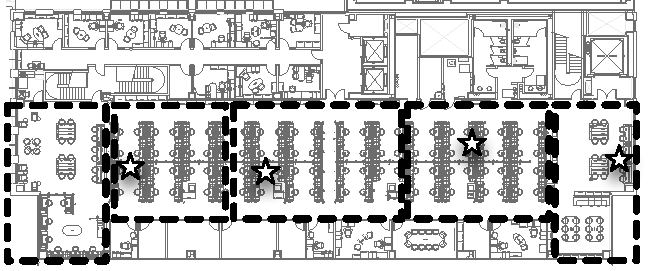
\includegraphics[width=.75\linewidth]{figs/floormap}
\end{center}
\caption{Location of routers shown in relation to actuation zones.}
\end{figure}

The routers cycle through each of the three wireless channels using tcpdump to capture packets in 1-second increments. Each packet is forwarded along with its 802.11 radiotap link-level header over SSH to a FIFO on the central computer, which parses out the RSSI and source MAC address. For each MAC address, for each time-step, for a given sample rate, each RSSI is converted to a linear scale and the resulting RSSIs are averaged per router. We can then compute the possible location $(x_d,y_d)$ of the device possessing a given MAC address as the centroid of the known router coordinates $(x_i, y_i)$ weighted by the average detected signal strength at that router $r_i$:
\begin{equation}
\begin{split}
x_d, y_d = \displaystyle\sum_{i} \frac{r_ix_i, r_iy_i}{\displaystyle\sum_i r_i}
\end{split}
\end{equation}
The central computer stores the 10 most recent computed centroids, and the location of the device is computed as the average of the 5 most closely clustered centroids of the 10 cached centroids (using Manhattan Distance as a heuristic). In practice, this ``averaging of averages'' greatly reduces the influence of the deployment environment upon the consistency of the measured RSSIs. Abnormally strong or weak signals thus do not alter the accuracy of our estimations. There is an incurred lag of about 4 times the sample rate should the device move, but this delay is acceptable within the bounds of accurate occupancy detection. We are able to place devices within 1 cubicle of their actual location. This level of precision is lower than for localization techniques that use training, but it is sufficient for counting people in HVAC or lighting zones which typically span 6-8 cubicles.

The passive nature of our localization infrastructure means that it requires little, if any, effort on behalf of the occupants to perform. It is only necessary for a device to associate with the available network before we can start tracking it. We can obtain a session IP address for a device with a given MAC address by listening to all wireless traffic. In the absence of regular or sufficient traffic, the central computer can occasionally ping the device in question to either elicit the requisite wireless traffic or determine if the device has left the tracking area (which suggests the user has left). This approach differs from previous wireless localization work in that it does not \emph{require} the user to ensure he/she is creating enough traffic to be localized accurately, but rather unobtrusively generates the necessary data. 

This raises the issue of accounting for ``detached devices,'' devices left connected to the network that are not actively being used and can therefore be falsely registered as occupants. The problem of detached devices can be addressed through analyzing packet and localization data. Network activity can be used as a proxy for human usage~\cite{Nedevschi2009}. For example, high-frequency HTTP traffic indicates likely human activity. Similarly, devices that move regularly are likely to indicate human presence. Conversely, devices that are always on and in a fixed location are likely to be desktops and are filtered out.

%The problem of detached devices can be approached with analysis of the specific types of packets sent by the device in question. For example, if the device is sending DHCP authentication packets, we can assume the device may have been associated with the given network for awhile but not logged-in, suggesting the device is not currently being used. Analysis of the number of HTTP packets for a given device can indicate the type and activity level of the device: low-frequency laptop traffic might suggest a detached device, whereas high-frequency mobile phone traffic implies an active user.

%In order to place an occupant within a space, it is necessary to have the routers form a convex hull of said space. Depending on the geometry of the space, fewer routers may be used to form a convex hull of lesser dimensionality that retains the domain of the zones of actuation. 

\begin{figure}[htb]
\begin{center}
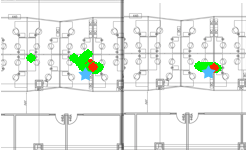
\includegraphics[width=.7\linewidth]{figs/samplesize}
\end{center}
\caption{Increased accuracy with increasingly large sample rates (20s, left; 10s, right). Even at times of low ambient signal noise, weighted centroid measurements can be inconsistent (black diamond), a problem remedied by averaging the 5 most closely clustered centroids (white circle). The star represents the actual device location.}
\end{figure}
